%!TEX root =  ../main.tex
\renewcommand{\columnseprule}{1.5pt}
\begin{multicols*}{2}
\rule[0.5\baselineskip]{0.4\textwidth}{1pt}
\noindent
\LabSection{Extremely Average}\label{sec:0205p}
\begin{exercises}{sec:0205p}

\lab{} The average rate of change of any function is simply the change in outputs, divided by the change in inputs.  For any function $f(x)$, write an algebraic fraction for the average rate of change from $c$ to $d$

\vspace{3cm}
\lab{} Next, suppose we want to find the average rate of change near point $c$.  Write out in correct notation, ``the limit as $x$ approaches $c$ of the average rate of change of $f(x)$ from $x$ to $c$''


\vspace{3cm}
\lab{} Coming out of the abstract, let us find the rate of change of a physical object, say a thrown ball.  A mathematical model for this situation might be $f(x)=-x2+4x+5$.  Begin by graphing the function in the first quadrant:

\noindent
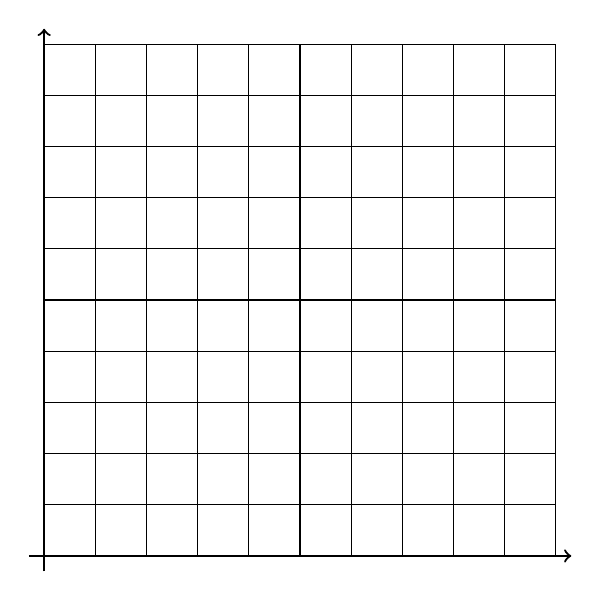
\begin{tikzpicture}[xscale=0.65,yscale=0.65]
	\draw [thick, ->] (-0.3,0) -- (10.3,0);
	\draw [thick, ->] (0,-0.3) -- (0,10.3);
	\draw [thin] (0,0) grid (10,10);
\end{tikzpicture}

\vspace{2cm}

\lab{}  If we try to calculate directly the average rate of change at 0, we get an indeterminate form.  Write the limit and solve it, for $x$ approaching 0 of the average rate of change of $f(x)$ from $x$ to 0.


\vspace{3cm}
\lab{} Looking at the graph, what do you estimate the rate of change is at $x=2$?  Use limits to find the answer.


\vspace{3cm}
\lab{}   When we are able to construct a function that outputs the rate of change, it is said to be the derivative function of the original.  Try to find the derivative of $f(x)$ by moving some distance $h$ to the right of $x$, setting up the average rate of change and taking the limit at $h$ approaches zero.


\vspace{5cm}
\lab{}  Describe in your own words what you think the point of this problem set is, using complete sentences.

\end{exercises}
\end{multicols*}